\documentclass[a4paper, 7.5pt]{extarticle}
\usepackage[utf8]{inputenc}
\usepackage[T1]{fontenc}
\usepackage{amsmath, amssymb, bm}
\usepackage{geometry}
\geometry{left=9mm, right=9mm, top=10mm, bottom=10mm}
\usepackage{tikz}
\usetikzlibrary{arrows.meta, positioning, calc, patterns, decorations.pathmorphing, decorations.markings}
\usepackage{tcolorbox}
\usepackage{multicol}
\usepackage{tabularx}
\usepackage{booktabs}
\usepackage{array}
\usepackage{xcolor}

\definecolor{boxblue}{RGB}{220,235,250}
\definecolor{boxtitle}{RGB}{30,80,150}
\definecolor{sketchgray}{RGB}{230,230,230}

\tcbset{
  colback=white, colframe=boxtitle, boxrule=0.6pt, arc=1pt,
  fonttitle=\bfseries\color{white}, coltitle=white, colbacktitle=boxtitle,
  top=2pt, bottom=2pt, left=3pt, right=3pt,
  toptitle=1pt, bottomtitle=1pt
}

\newcommand{\unitbox}[1]{\textnormal{\small\textcolor{boxtitle}{\textbf{[#1]}}}}
\newcommand{\vardef}[2]{\(#1\): #2}

\setlength{\parindent}{0pt}
\setlength{\parskip}{0.3ex}
\setlength{\columnsep}{4mm}

\begin{document}

\begin{center}
    \textbf{\Large Formelsammlung: Elektromagnetische Felder}\\[1pt]
    \textit{Mit Einheiten, Variablenbedeutungen, Betrachtungspunkten und Skizzen}
\end{center}

\begin{multicols*}{2}

%=============================================================
\section*{1. Mathematische Grundlagen}
%=============================================================

\begin{tcolorbox}[title={Maxwell-Gleichungen -- Differentiell \& Integral}]
\textbf{Differentialform:}\\
$\text{rot}\,\vec{E} = -\dfrac{\partial \vec{B}}{\partial t}$\quad
$\text{div}\,\vec{B} = 0$\\[2pt]
$\text{rot}\,\vec{H} = \vec{J} + \dfrac{\partial \vec{D}}{\partial t}$\quad
$\text{div}\,\vec{D} = \rho_V$\\[3pt]
\textbf{Integralform:}\\
$\oint \vec{E}\cdot d\vec{s} = -\dfrac{d}{dt}\iint \vec{B}\cdot d\vec{A}$ \quad (Faraday)\\[2pt]
$\oint \vec{H}\cdot d\vec{s} = I_{enc} + \dfrac{d}{dt}\iint \vec{D}\cdot d\vec{A}$ \quad (Ampère)\\[2pt]
$\oint \vec{D}\cdot d\vec{A} = Q_{enc}$\quad (Gauß)\\[2pt]
$\oint \vec{B}\cdot d\vec{A} = 0$\quad (kein mag. Monopol)\\[3pt]
\textbf{Materialgleichungen:}\\
$\vec{D} = \varepsilon_0\varepsilon_r\vec{E}$ \;\text{\textcolor{boxtitle}{[\(As/m^2\)]}}\quad
$\vec{B} = \mu_0\mu_r\vec{H}$ \;\text{\textcolor{boxtitle}{[\(T = Vs/m^2\)]}}\\
$\vec{J} = \kappa\vec{E}$ \;\text{\textcolor{boxtitle}{[\(A/m^2\)]}}\\[3pt]
\textbf{Konstanten:}\\
$\varepsilon_0 = 8{,}854\cdot10^{-12}$ \;\text{\textcolor{boxtitle}{[\(As/(Vm) = F/m\)]}}\\
$\mu_0 = 4\pi\cdot10^{-7}$ \;\text{\textcolor{boxtitle}{[\(Vs/(Am) = H/m\)]}}\\
$c = 1/\sqrt{\mu_0\varepsilon_0} = 2{,}998\cdot10^8$ \;\text{\textcolor{boxtitle}{[\(m/s\)]}}\\
$Z_0 = \sqrt{\mu_0/\varepsilon_0} = 377$ \;\text{\textcolor{boxtitle}{[\(\Omega\)]}}
\end{tcolorbox}

\begin{tcolorbox}[title={Koordinatensysteme \& Volumenelemente}]
\begin{center}
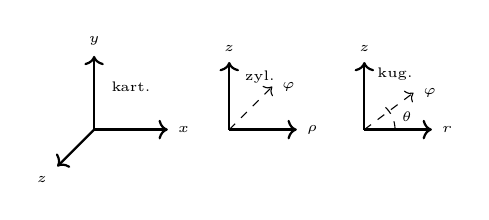
\begin{tikzpicture}[scale=0.78]
  % Kartesisch
  \draw[->,thick] (0,0,0) -- (1.2,0,0) node[right]{\tiny$x$};
  \draw[->,thick] (0,0,0) -- (0,1.2,0) node[above]{\tiny$y$};
  \draw[->,thick] (0,0,0) -- (-0.6,-0.6,0) node[below left]{\tiny$z$};
  \node at (0.6,0.7) {\tiny kart.};
  % Zylindrisch
  \begin{scope}[xshift=2.2cm]
    \draw[->,thick] (0,0) -- (1.1,0) node[right]{\tiny$\rho$};
    \draw[->,thick] (0,0) -- (0,1.1) node[above]{\tiny$z$};
    \draw[->,dashed] (0,0) -- (0.7,0.7) node[right]{\tiny$\varphi$};
    \node at (0.5,0.85) {\tiny zyl.};
  \end{scope}
  % Kugel
  \begin{scope}[xshift=4.4cm]
    \draw[->,thick] (0,0) -- (1.1,0) node[right]{\tiny$r$};
    \draw[->,thick] (0,0) -- (0,1.1) node[above]{\tiny$z$};
    \draw[->,dashed] (0,0) -- (0.8,0.6) node[right]{\tiny$\varphi$};
    \draw[dashed] (0.5,0) arc(0:50:0.5) node[midway, right]{\tiny$\theta$};
    \node at (0.5,0.9) {\tiny kug.};
  \end{scope}
\end{tikzpicture}
\end{center}
\textbf{Kartesisch $(x,y,z)$:}\quad $dV = dx\,dy\,dz$\\
\textbf{Zylinder $(\rho,\varphi,z)$:}\quad $x=\rho\cos\varphi$, $y=\rho\sin\varphi$\\
$dV = \rho\,d\rho\,d\varphi\,dz$;\quad $d\vec{A}_\rho = \rho\,d\varphi\,dz\,\vec{e}_\rho$\\
\textbf{Kugel $(r,\theta,\varphi)$:}\quad $x=r\sin\theta\cos\varphi$, $y=r\sin\theta\sin\varphi$\\
$z=r\cos\theta$;\quad $dV = r^2\sin\theta\,dr\,d\theta\,d\varphi$\\
$d\vec{A}_r = r^2\sin\theta\,d\theta\,d\varphi\,\vec{e}_r$
\end{tcolorbox}

\begin{tcolorbox}[title={Differentialoperatoren -- alle Koordinatensysteme}]
\textbf{Gradient} $\nabla\phi$ \;\text{\textcolor{boxtitle}{[\(V/m\)]}} \quad(Skalar $\to$ Vektor, zeigt in Richtung stärksten Anstiegs):
$$\nabla\phi\big|_{\text{kart}} = \partial_x\phi\,\vec{e}_x + \partial_y\phi\,\vec{e}_y + \partial_z\phi\,\vec{e}_z$$
$$\nabla\phi\big|_{\text{zyl}} = \partial_\rho\phi\,\vec{e}_\rho + \tfrac{1}{\rho}\partial_\varphi\phi\,\vec{e}_\varphi + \partial_z\phi\,\vec{e}_z$$
$$\nabla\phi\big|_{\text{kug}} = \partial_r\phi\,\vec{e}_r + \tfrac{1}{r}\partial_\theta\phi\,\vec{e}_\theta + \tfrac{1}{r\sin\theta}\partial_\varphi\phi\,\vec{e}_\varphi$$
\textbf{Divergenz} $\nabla\cdot\vec{F}$ \unitbox{1/m $\cdot$ [F]} \quad(Vektor $\to$ Skalar, Quellstärke):
$$\nabla\cdot\vec{F}\big|_{\text{kart}} = \partial_x F_x + \partial_y F_y + \partial_z F_z$$
$$\nabla\cdot\vec{F}\big|_{\text{zyl}} = \tfrac{1}{\rho}\partial_\rho(\rho F_\rho) + \tfrac{1}{\rho}\partial_\varphi F_\varphi + \partial_z F_z$$
$$\nabla\cdot\vec{F}\big|_{\text{kug}} = \tfrac{1}{r^2}\partial_r(r^2 F_r) + \tfrac{1}{r\sin\theta}\partial_\theta(\sin\theta F_\theta) + \tfrac{1}{r\sin\theta}\partial_\varphi F_\varphi$$
\textbf{Rotation} $\nabla\times\vec{F}$ \unitbox{1/m $\cdot$ [F]} \quad(Vektor $\to$ Vektor, Wirbelstärke):
$$(\nabla\times\vec{F})_x = \partial_y F_z - \partial_z F_y$$
$$(\nabla\times\vec{F})_y = \partial_z F_x - \partial_x F_z$$
$$(\nabla\times\vec{F})_z = \partial_x F_y - \partial_y F_x$$
\textbf{Laplace-Operator} $\Delta\phi = \nabla\cdot(\nabla\phi)$:
$$\Delta\phi\big|_{\text{kart}} = \partial_x^2\phi + \partial_y^2\phi + \partial_z^2\phi$$
$$\Delta\phi\big|_{\text{zyl}} = \tfrac{1}{\rho}\partial_\rho(\rho\,\partial_\rho\phi) + \tfrac{1}{\rho^2}\partial_\varphi^2\phi + \partial_z^2\phi$$
$$\Delta\phi\big|_{\text{kug}} = \tfrac{1}{r^2}\partial_r(r^2\partial_r\phi) + \tfrac{1}{r^2\sin\theta}\partial_\theta(\sin\theta\,\partial_\theta\phi) + \tfrac{1}{r^2\sin^2\theta}\partial_\varphi^2\phi$$
\end{tcolorbox}

\begin{tcolorbox}[title={Integralsätze \& Vektoridentitäten}]
\textbf{Gaußscher Satz} (Volumen $V$, Hülle $\partial V$):
$$\oint_{\partial V}\vec{F}\cdot d\vec{A} = \int_V \nabla\cdot\vec{F}\,dV$$
\textbf{Stokesscher Satz} (Fläche $A$, Rand $\partial A$):
$$\oint_{\partial A}\vec{F}\cdot d\vec{s} = \int_A (\nabla\times\vec{F})\cdot d\vec{A}$$
\textbf{Wichtige Identitäten:}\\
$\nabla\times(\nabla\phi) = \vec{0}$\quad(Gradient ist wirbelfrei)\\
$\nabla\cdot(\nabla\times\vec{F}) = 0$\quad(Rotation ist quellenfrei)\\
$\nabla\times(\nabla\times\vec{F}) = \nabla(\nabla\cdot\vec{F}) - \Delta\vec{F}$\\
$\text{grad}\,r = \vec{r}/r$;\quad $\text{grad}(1/r) = -\vec{r}/r^3$\\
$\text{div}\,\vec{r} = 3$;\quad $\text{div}(\vec{r}/r^3) = 0$ (für $r\neq0$)\\
$\text{rot}\,\vec{r} = \vec{0}$;\quad $\text{div}(\vec{r}/r) = 2/r$
\end{tcolorbox}

\begin{tcolorbox}[title={Delta-Funktion $\delta(\vec{r})$ -- Punktquelle}]
\textbf{Definition:} $\delta(x)=0$ für $x\neq0$;\quad $\int_{-\infty}^{+\infty}\delta(x)\,dx=1$\\
\textbf{3D:} $\delta(\vec{r}) = \delta(x)\delta(y)\delta(z)$ \;\text{\textcolor{boxtitle}{[\(1/m^3\)]}}\\
\textbf{Ausblendeigenschaft:}
$$\int_{-\infty}^{+\infty} f(x)\,\delta(x-x_0)\,dx = f(x_0)$$
\textbf{Punktladung} am Ort $\vec{r}_0$:
$\rho_V(\vec{r}) = Q\,\delta(\vec{r}-\vec{r}_0)$ \;\text{\textcolor{boxtitle}{[\(C/m^3\)]}}
\end{tcolorbox}

\begin{tcolorbox}[title={Helmholtz-Theorem \& Eindeutigkeit}]
Jedes Vektorfeld $\vec{F}$ ist durch Divergenz + Rotation \textbf{eindeutig} bestimmt:
$$\vec{F} = \underbrace{-\text{grad}\,\phi}_{\text{quellbehaftet}} + \underbrace{\text{rot}\,\vec{A}}_{\text{wirbelbehaftet}}$$
$\phi$ = Skalarpotential \;\text{\textcolor{boxtitle}{[\(V\)]}};\quad $\vec{A}$ = Vektorpotential \;\text{\textcolor{boxtitle}{[\(Vs/m\)]}}\\[3pt]
\textbf{Eindeutigkeit der Lösung:} Wenn auf dem Rand $\partial V$ überall $\phi$ (Dirichlet) \textit{oder} $\partial\phi/\partial n$ (Neumann) vorgegeben ist $\Rightarrow$ \textbf{eindeutige} Lösung.
\end{tcolorbox}

\begin{tcolorbox}[title={Einteilung elektromagnetischer Felder}]
\begin{tabular}{@{}lll@{}}
\toprule
Feldtyp & Bedingung & Hauptgleichung\\
\midrule
Elektrostatik & $\partial_t=0$, $\vec{J}=0$ & Laplace/Poisson\\
Strömungsfeld & $\partial_t=0$, $\vec{J}\neq0$ & $\Delta\phi=0$\\
Magnetostatik & $\partial_t=0$ & Ampère\\
EQS & $\partial_t\vec{B}\approx0$ & Poisson (kompl.)\\
MQS & $\partial_t\vec{D}\approx0$ & Diffusionsgl.\\
Volle Maxwell & allgemein & Wellengleichung\\
\bottomrule
\end{tabular}
\end{tcolorbox}

%=============================================================
\section*{2. Elektrostatik}
%=============================================================

\begin{tcolorbox}[title={Grundgleichungen Elektrostatik}]
$\text{rot}\,\vec{E} = 0 \Rightarrow \oint\vec{E}\cdot d\vec{s} = 0$\quad (wirbelfrei)\\
$\vec{E} = -\text{grad}\,\phi$\quad \;\text{\textcolor{boxtitle}{[\(V/m\)]}}\\
$\text{div}\,\vec{D} = \rho_V \Rightarrow \oint\vec{D}\cdot d\vec{A} = Q_{enc}$\\
\textbf{Poisson:} $\Delta\phi = -\rho_V/\varepsilon$\quad \;\text{\textcolor{boxtitle}{[\(V/m^2\)]}}\\
\textbf{Laplace:} $\Delta\phi = 0$ (ladungsfrei)\\
Coulombkraft: $\vec{F} = q\vec{E}$ \;\text{\textcolor{boxtitle}{[\(N\)]}}\\
Spannung: $U_{21} = \phi_2-\phi_1 = -\int_1^2\vec{E}\cdot d\vec{s}$ \;\text{\textcolor{boxtitle}{[\(V\)]}}
\end{tcolorbox}

\begin{tcolorbox}[title={Potentialberechnung -- 3 Methoden}]
\textbf{Methode 1: Wegintegral} (wenn $\vec{E}$ bekannt):
$$\phi(\vec{r}) = -\int_{\vec{r}_0}^{\vec{r}}\vec{E}\cdot d\vec{s} + \phi(\vec{r}_0)$$
\textbf{Methode 2: Laplace/Poisson lösen:}\\
\phantom{x}1. Symmetrie $\Rightarrow$ Koordinatenabhängigkeit\\
\phantom{x}2. Zweimal integrieren $\Rightarrow$ $C_1, C_2$\\
\phantom{x}3. Randbedingungen einsetzen\\[3pt]
\textbf{Methode 3: Superpositionsintegral:}
$$\phi(\vec{r}) = \frac{1}{4\pi\varepsilon_0}\int_{V'}\frac{\rho_V(\vec{r}')}{|\vec{r}-\vec{r}'|}\,dV'$$
\end{tcolorbox}

\begin{tcolorbox}[title={Punktladung}]
\begin{center}
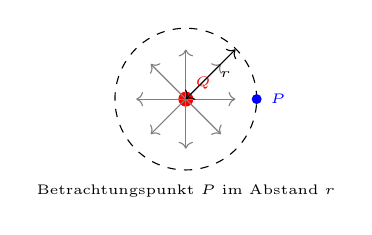
\begin{tikzpicture}[scale=0.9]
  \fill[red] (0,0) circle (3pt) node[above right]{\tiny$Q$};
  \foreach \a in {0,45,...,315}
    \draw[->,gray] (0,0) -- ({0.7*cos(\a)},{0.7*sin(\a)});
  \draw[dashed] (0,0) circle (1cm);
  \draw[<->] (0,0) -- (0.7,0.7) node[midway,right]{\tiny$r$};
  \node[blue] at (1.3,0) {\tiny$P$};
  \fill[blue] (1.0,0) circle (2pt);
  \node at (0,-1.3) {\tiny Betrachtungspunkt $P$ im Abstand $r$};
\end{tikzpicture}
\end{center}
$$\vec{E}(r) = \frac{Q}{4\pi\varepsilon r^2}\vec{e}_r \;\text{\textcolor{boxtitle}{[\(V/m\)]}},\quad \phi(r) = \frac{Q}{4\pi\varepsilon r} \;\text{\textcolor{boxtitle}{[\(V\)]}}$$
$r$ \;\text{\textcolor{boxtitle}{[\(m\)]}}: Abstand von $Q$ zum Aufpunkt $P$\\
$\varepsilon = \varepsilon_0\varepsilon_r$ \;\text{\textcolor{boxtitle}{[\(As/(Vm)\)]}}: Permittivität des Mediums\\
$\vec{e}_r$: Einheitsvektor von $Q$ nach $P$
\end{tcolorbox}

\begin{tcolorbox}[title={Unendliche Linienladung}]
\begin{center}
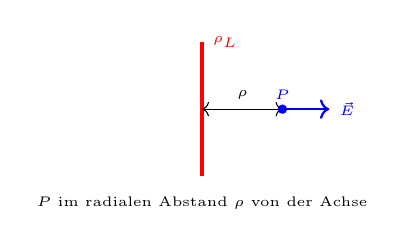
\begin{tikzpicture}[scale=0.85]
  \draw[very thick, red] (0,-1) -- (0,1) node[right]{\tiny$\rho_L$};
  \draw[<->] (0,0) -- (1.2,0) node[midway,above]{\tiny$\rho$};
  \draw[->,blue,thick] (1.2,0) -- (1.9,0) node[right]{\tiny$\vec{E}$};
  \fill[blue] (1.2,0) circle (2pt) node[above]{\tiny$P$};
  \node at (0,-1.4) {\tiny $P$ im radialen Abstand $\rho$ von der Achse};
\end{tikzpicture}
\end{center}
$$\vec{E}(\rho) = \frac{\rho_L}{2\pi\varepsilon\rho}\vec{e}_\rho \;\text{\textcolor{boxtitle}{[\(V/m\)]}}$$
$$\phi(\rho) = -\frac{\rho_L}{2\pi\varepsilon}\ln\!\left(\frac{\rho}{\rho_0}\right) \;\text{\textcolor{boxtitle}{[\(V\)]}}$$
$\rho_L$ \;\text{\textcolor{boxtitle}{[\(C/m\)]}}: Linienladungsdichte\\
$\rho$ \;\text{\textcolor{boxtitle}{[\(m\)]}}: radialer Abstand von der Achse\\
$\rho_0$: Bezugsabstand mit $\phi(\rho_0)=0$
\end{tcolorbox}

\begin{tcolorbox}[title={Unendliche Flächenladung}]
\begin{center}
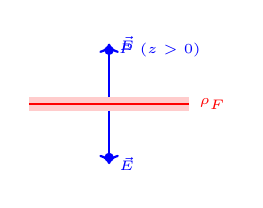
\begin{tikzpicture}[scale=0.85]
  \fill[red!20] (-1.2,-0.1) rectangle (1.2,0.1);
  \draw[red, thick] (-1.2,0) -- (1.2,0) node[right]{\tiny$\rho_F$};
  \draw[->,blue,thick] (0,0.1) -- (0,0.9) node[right]{\tiny$\vec{E}$};
  \draw[->,blue,thick] (0,-0.1) -- (0,-0.9) node[right]{\tiny$\vec{E}$};
  \fill[blue] (0,0.8) circle (2pt) node[right]{\tiny$P$ ($z>0$)};
  \fill[blue] (0,-0.8) circle (2pt);
\end{tikzpicture}
\end{center}
$$\vec{E} = \frac{\rho_F}{2\varepsilon}\vec{n} \;\text{\textcolor{boxtitle}{[\(V/m\)]}},\quad \phi(z) = -\frac{\rho_F}{2\varepsilon}|z| \;\text{\textcolor{boxtitle}{[\(V\)]}}$$
$\rho_F$ \;\text{\textcolor{boxtitle}{[\(C/m^2\)]}}: Flächenladungsdichte\\
$\vec{n}$: Normalenvektor von der Fläche weg\\
$P$ liegt im Abstand $|z|$ von der Fläche
\end{tcolorbox}

\begin{tcolorbox}[title={Raumladungskugel (homogen)}]
\begin{center}
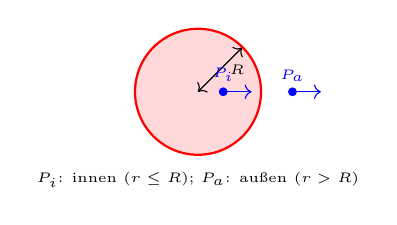
\begin{tikzpicture}[scale=0.8]
  \fill[red!15] (0,0) circle (1cm);
  \draw[red,thick] (0,0) circle (1cm);
  \draw[<->] (0,0) -- (0.7,0.7) node[midway,right]{\tiny$R$};
  % innen
  \fill[blue] (0.4,0) circle (2pt) node[above]{\tiny$P_i$};
  \draw[->,blue] (0.4,0) -- (0.85,0);
  % außen
  \fill[blue] (1.5,0) circle (2pt) node[above]{\tiny$P_a$};
  \draw[->,blue] (1.5,0) -- (1.95,0);
  \node at (0,-1.4) {\tiny$P_i$: innen ($r\leq R$); $P_a$: außen ($r>R$)};
\end{tikzpicture}
\end{center}
\textbf{Innen} ($r\leq R$, Betrachtungspunkt $P_i$):
$$\vec{E} = \frac{\rho_V r}{3\varepsilon}\vec{e}_r,\quad \phi = \frac{\rho_V}{6\varepsilon}(3R^2-r^2)$$
\textbf{Außen} ($r>R$, Betrachtungspunkt $P_a$):
$$\vec{E} = \frac{\rho_V R^3}{3\varepsilon r^2}\vec{e}_r,\quad \phi = \frac{\rho_V R^3}{3\varepsilon r}$$
$\rho_V$ \;\text{\textcolor{boxtitle}{[\(C/m^3\)]}}: Volumenladungsdichte;\quad $R$ \;\text{\textcolor{boxtitle}{[\(m\)]}}: Kugelradius
\end{tcolorbox}

\begin{tcolorbox}[title={Geladener Kreisring \& Kreisscheibe (z-Achse)}]
\begin{center}
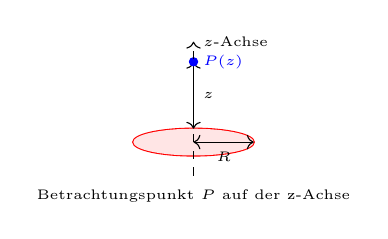
\begin{tikzpicture}[scale=0.85]
  \draw[red,thick] (0,0) ellipse (0.9cm and 0.2cm);
  \fill[red!10] (0,0) ellipse (0.9cm and 0.2cm);
  \draw[<->] (0,0) -- (0.9,0) node[midway,below]{\tiny$R$};
  \draw[<->] (0,0.2) -- (0,1.2) node[midway,right]{\tiny$z$};
  \fill[blue] (0,1.2) circle (2pt) node[right]{\tiny$P(z)$};
  \draw[dashed,->] (0,-0.5) -- (0,1.5) node[right]{\tiny$z$-Achse};
  \node at (0,-0.8) {\tiny Betrachtungspunkt $P$ auf der z-Achse};
\end{tikzpicture}
\end{center}
\textbf{Kreisring} (Gesamtladung $Q$):
$$\vec{E}(z) = \frac{Qz}{4\pi\varepsilon(R^2+z^2)^{3/2}}\vec{e}_z$$
\textbf{Kreisscheibe} (Flächenladung $\rho_F$, $z>0$):
$$\phi(z) = \frac{\rho_F}{2\varepsilon_0}(\sqrt{R^2+z^2}-|z|)$$
$$\vec{E}(z) = \frac{\rho_F}{2\varepsilon}\!\left(1-\frac{z}{\sqrt{R^2+z^2}}\right)\vec{e}_z$$
$z$ \;\text{\textcolor{boxtitle}{[\(m\)]}}: Abstand des Aufpunkts vom Mittelpunkt entlang der z-Achse
\end{tcolorbox}

\begin{tcolorbox}[title={Elektrischer Dipol (Fernfeld)}]
\begin{center}
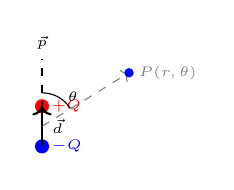
\begin{tikzpicture}[scale=0.85]
  \fill[blue] (0,-0.3) circle (3pt) node[right]{\tiny$-Q$};
  \fill[red] (0,0.3) circle (3pt) node[right]{\tiny$+Q$};
  \draw[->,thick] (0,-0.3) -- (0,0.3) node[midway,right]{\tiny$\vec{d}$};
  \draw[dashed,->,gray] (0,0) -- (1.3,0.8) node[right]{\tiny$P(r,\theta)$};
  \fill[blue] (1.3,0.8) circle (2pt);
  \draw[dashed] (0,0) -- (0,1) node[above]{\tiny$\vec{p}$};
  \draw (0,0.5) arc(90:33:0.5) node[midway,right]{\tiny$\theta$};
\end{tikzpicture}
\end{center}
Dipolmoment: $\vec{p} = Q\vec{d}$ \;\text{\textcolor{boxtitle}{[\(Cm\)]}}\\[3pt]
Fernfeld ($r\gg d$), Betrachtungspunkt in Kugelkoordinaten:
$$\phi(r,\theta) = \frac{p\cos\theta}{4\pi\varepsilon r^2},\quad E_r = \frac{2p\cos\theta}{4\pi\varepsilon r^3},\quad E_\theta = \frac{p\sin\theta}{4\pi\varepsilon r^3}$$
$r$ \;\text{\textcolor{boxtitle}{[\(m\)]}}: Abstand vom Dipolmittelpunkt;\quad $\theta$: Winkel zur Dipolachse
\end{tcolorbox}

\begin{tcolorbox}[title={Grenzbedingungen Elektrostatik}]
\begin{center}
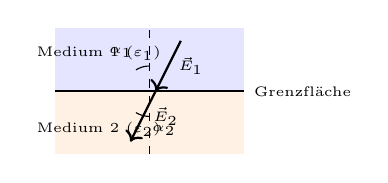
\begin{tikzpicture}[scale=0.8]
  \fill[blue!10] (-1.5,0) rectangle (1.5,1);
  \fill[orange!10] (-1.5,-1) rectangle (1.5,0);
  \draw[thick] (-1.5,0) -- (1.5,0) node[right]{\tiny Grenzfläche};
  \node at (-0.8,0.6) {\tiny Medium 1 ($\varepsilon_1$)};
  \node at (-0.8,-0.6) {\tiny Medium 2 ($\varepsilon_2$)};
  \draw[->,thick] (0.5,0.8) -- (0.1,0) node[midway,right]{\tiny$\vec{E}_1$};
  \draw[->,thick] (0.1,0) -- (-0.3,-0.8) node[midway,right]{\tiny$\vec{E}_2$};
  \draw[dashed] (0,-1) -- (0,1);
  \draw (0,0.4) arc(90:122:0.4) node[midway,above left]{\tiny$\alpha_1$};
  \draw (0,-0.4) arc(270:238:0.4) node[midway,below right]{\tiny$\alpha_2$};
\end{tikzpicture}
\end{center}
\textbf{Tangential:} $E_{1t} = E_{2t}$ (E-Feld stetig)\\
\textbf{Normal:} $D_{2n} - D_{1n} = \rho_F$ \;\text{\textcolor{boxtitle}{[\(C/m^2\)]}}\\
Ohne freie Ladung ($\rho_F=0$): $\varepsilon_1 E_{1n} = \varepsilon_2 E_{2n}$\\[3pt]
\textbf{Brechungsgesetz:} $\dfrac{\tan\alpha_1}{\tan\alpha_2} = \dfrac{\varepsilon_1}{\varepsilon_2}$\\[3pt]
\textbf{An Leiteroberfläche} ($\kappa\to\infty$): $E_t = 0$, $D_n = \rho_F$, $\phi=\text{const}$
\end{tcolorbox}

\begin{tcolorbox}[title={Kapazitäten -- alle Geometrien}]
$C = Q/U$ \;\text{\textcolor{boxtitle}{[\(F = As/V\)]}};\quad Energie: $W_e = \tfrac{1}{2}CU^2$ \;\text{\textcolor{boxtitle}{[\(J\)]}}
$$W_e = \frac{1}{2}\int_V\varepsilon E^2\,dV = \frac{Q^2}{2C}$$
\textbf{Plattenkondensator:}\quad $C = \varepsilon A/d$\\
\phantom{x}$A$ \;\text{\textcolor{boxtitle}{[\(m^2\)]}}: Plattenfläche;\quad $d$ \;\text{\textcolor{boxtitle}{[\(m\)]}}: Plattenabstand\\[2pt]
\textbf{Zylinderkondensator:}\quad $C = 2\pi\varepsilon l/\ln(r_a/r_i)$\\
\phantom{x}$r_i, r_a$ \;\text{\textcolor{boxtitle}{[\(m\)]}}: Innen-/Außenradius;\quad $l$ \;\text{\textcolor{boxtitle}{[\(m\)]}}: Länge\\[2pt]
\textbf{Kugelkondensator:}\quad $C = 4\pi\varepsilon r_i r_a/(r_a-r_i)$\\[2pt]
\textbf{Einzelkugel} ($r_a\to\infty$):\quad $C = 4\pi\varepsilon r_i$\\[3pt]
\textbf{Reihenschaltung} (Lagen $\parallel$ zu Elektroden):
$\;1/C_{ges} = \sum 1/C_i$\\
\textbf{Parallelschaltung} (Lagen $\perp$ zu Elektroden):
$\;C_{ges} = \sum C_i$
\end{tcolorbox}

\begin{tcolorbox}[title={Spiegelungsmethode}]
\begin{center}
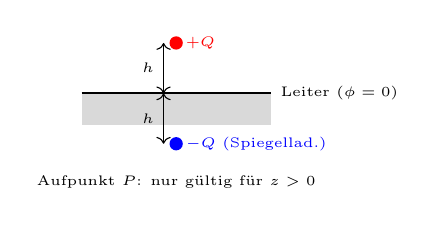
\begin{tikzpicture}[scale=0.8]
  \fill[gray!30] (-1.5,-0.5) rectangle (1.5,0);
  \draw[thick] (-1.5,0) -- (1.5,0) node[right]{\tiny Leiter ($\phi=0$)};
  \fill[red] (0,0.8) circle (3pt) node[right]{\tiny$+Q$};
  \fill[blue] (0,-0.8) circle (3pt) node[right]{\tiny$-Q$ (Spiegellad.)};
  \draw[<->] (-0.2,0) -- (-0.2,0.8) node[midway,left]{\tiny$h$};
  \draw[<->] (-0.2,0) -- (-0.2,-0.8) node[midway,left]{\tiny$h$};
  \node at (0,-1.4) {\tiny Aufpunkt $P$: nur gültig für $z>0$};
\end{tikzpicture}
\end{center}
$$\phi(\vec{r}) = \frac{1}{4\pi\varepsilon}\!\left(\frac{Q}{r_+} - \frac{Q}{r_-}\right) \;\text{\textcolor{boxtitle}{[\(V\)]}}$$
$r_+$: Abstand zu $+Q$;\quad $r_-$: Abstand zur Spiegelladung\\
Induzierte Oberflächenladung: $\rho_F = \varepsilon\,E_n\big|_{\text{Oberfläche}}$\\
Kraft auf $Q$ im Abstand $h$: $F = Q^2/[4\pi\varepsilon(2h)^2]$ (anziehend)
\end{tcolorbox}

%=============================================================
\section*{3. Stationäres Strömungsfeld}
%=============================================================

\begin{tcolorbox}[title={Grundgleichungen \& Einheiten}]
$\vec{J} = \kappa\vec{E}$ \;\text{\textcolor{boxtitle}{[\(A/m^2\)]}}\quad (Ohmsches Gesetz, differentiell)\\
$\text{div}\,\vec{J} = 0 \Rightarrow \oint\vec{J}\cdot d\vec{A} = 0$ \quad (Kontinuität)\\
$\text{rot}\,\vec{E} = 0 \Rightarrow \Delta\phi = 0$ \quad (Laplace)\\
$R = U/I$ \;\text{\textcolor{boxtitle}{[\(\Omega\)]}};\quad $p = \vec{J}\cdot\vec{E} = \kappa E^2$ \;\text{\textcolor{boxtitle}{[\(W/m^3\)]}}\\
Leistung: $P = UI = I^2R$ \;\text{\textcolor{boxtitle}{[\(W\)]}}\\[2pt]
\textbf{Variablen:}\quad
$\kappa$ \;\text{\textcolor{boxtitle}{[\(S/m\)]}}: Leitfähigkeit;\quad $\rho=1/\kappa$ \;\text{\textcolor{boxtitle}{[\(\Omega m\)]}}: spez. Widerstand
\end{tcolorbox}

\begin{tcolorbox}[title={Widerstände -- alle Geometrien}]
\begin{center}
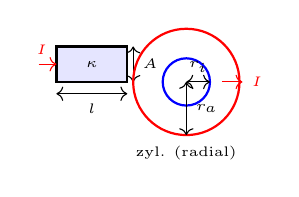
\begin{tikzpicture}[scale=0.75]
  % Quader
  \fill[blue!10] (0,0) rectangle (1.2,0.6);
  \draw[thick] (0,0) rectangle (1.2,0.6);
  \draw[<->] (0,-0.2) -- (1.2,-0.2) node[midway,below]{\tiny$l$};
  \draw[<->] (1.3,0) -- (1.3,0.6) node[midway,right]{\tiny$A$};
  \draw[->,red] (-0.3,0.3) -- (0,0.3) node[above left]{\tiny$I$};
  \node at (0.6,0.3) {\tiny$\kappa$};
  % Zylinder
  \begin{scope}[xshift=2.2cm]
    \draw[red,thick] (0,0) circle (0.9cm);
    \draw[blue,thick] (0,0) circle (0.4cm);
    \draw[<->] (0,0) -- (0.4,0) node[midway,above]{\tiny$r_i$};
    \draw[<->] (0,0) -- (0,-0.9) node[midway,right]{\tiny$r_a$};
    \draw[->,red] (0.6,0) -- (0.95,0) node[right]{\tiny$I$};
    \node at (0,-1.2) {\tiny zyl. (radial)};
  \end{scope}
\end{tikzpicture}
\end{center}
\textbf{Quader:} $R = l/(\kappa A)$\quad ($l$: Länge, $A$: Querschnitt)\\[2pt]
\textbf{Zylinderschale} (radialer Strom):
$$R = \frac{1}{2\pi\kappa l}\ln\!\left(\frac{r_a}{r_i}\right) \;\text{\textcolor{boxtitle}{[\(\Omega\)]}}$$
\textbf{Kugelschale} (radialer Strom):
$$R = \frac{1}{4\pi\kappa}\!\left(\frac{1}{r_i} - \frac{1}{r_a}\right)$$
\textbf{Halbkugelerder} (Radius $a$): $R = 1/(2\pi\kappa a)$\\[2pt]
\textbf{Kreisbogen} (azimutaler Strom, Winkel $\alpha$, Breite $b$):
$$R = \frac{\alpha}{\kappa b\ln(r_a/r_i)}$$
\textbf{Kegelstumpf} (Radien $R_1, R_2$, Höhe $h$):
$$R = \frac{h}{\kappa\pi R_1 R_2}$$
\textbf{Variabler Querschnitt} $A(x)=A_0(\frac{\alpha-1}{l}x+1)$:
$$R = \frac{l}{\kappa A_0(\alpha-1)}\ln(\alpha)$$
\end{tcolorbox}

\begin{tcolorbox}[title={Geschichtete Medien (Strömungsfeld)}]
\begin{center}
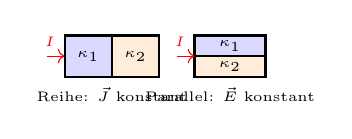
\begin{tikzpicture}[scale=0.75]
  % Reihe
  \fill[blue!15] (0,0) rectangle (0.8,0.7);
  \fill[orange!15] (0.8,0) rectangle (1.6,0.7);
  \draw[thick] (0,0) rectangle (1.6,0.7);
  \draw[thick] (0.8,0) -- (0.8,0.7);
  \node at (0.4,0.35) {\tiny$\kappa_1$};
  \node at (1.2,0.35) {\tiny$\kappa_2$};
  \draw[->,red] (-0.3,0.35) -- (0,0.35) node[above left]{\tiny$I$};
  \node at (0.8,-0.3) {\tiny Reihe: $\vec{J}$ konstant};
  % Parallel
  \begin{scope}[xshift=2.2cm]
    \fill[blue!15] (0,0.35) rectangle (1.2,0.7);
    \fill[orange!15] (0,0) rectangle (1.2,0.35);
    \draw[thick] (0,0) rectangle (1.2,0.7);
    \draw[thick] (0,0.35) -- (1.2,0.35);
    \node at (0.6,0.52) {\tiny$\kappa_1$};
    \node at (0.6,0.17) {\tiny$\kappa_2$};
    \draw[->,red] (-0.3,0.35) -- (0,0.35) node[above left]{\tiny$I$};
    \node at (0.6,-0.3) {\tiny Parallel: $\vec{E}$ konstant};
  \end{scope}
\end{tikzpicture}
\end{center}
\textbf{Reihe} (quer zur Stromrichtung, $\vec{J}$ gleich):
$$R_{ges} = \sum_i\frac{l_i}{\kappa_i A}$$
\textbf{Parallel} (längs zur Stromrichtung, $\vec{E}$ gleich):
$$\frac{1}{R_{ges}} = \sum_i\frac{\kappa_i A_i}{l}$$
\textbf{Grenzbedingungen:}\\
\phantom{x}Tangential: $E_{1t} = E_{2t}$\quad (E stetig)\\
\phantom{x}Normal: $J_{1n} = J_{2n}$\quad (J stetig)\\[2pt]
\textbf{Koaxial, vertikal geschichtet:}
$$R = \frac{\ln(\rho_a/\rho_i)}{2\pi(l_1\kappa_1+l_2\kappa_2)}$$
\textbf{Analogie} $C\cdot R = \varepsilon/\kappa$ (gleiche Geometrie)
\end{tcolorbox}

%=============================================================
\section*{4. Magnetostatik}
%=============================================================

\begin{tcolorbox}[title={Grundgleichungen Magnetostatik}]
$\text{div}\,\vec{B} = 0 \Rightarrow \oint\vec{B}\cdot d\vec{A} = 0$ \;\text{\textcolor{boxtitle}{[\(T = Vs/m^2\)]}}\\
$\text{rot}\,\vec{H} = \vec{J} \Rightarrow \oint\vec{H}\cdot d\vec{s} = I_{enc}$ \;\text{\textcolor{boxtitle}{[\(A/m\)]}}\\
$\vec{B} = \mu_0\mu_r\vec{H}$;\quad $\vec{B} = \text{rot}\,\vec{A}$ \;\text{\textcolor{boxtitle}{[\(T\)]}}\\
$\Delta\vec{A} = -\mu\vec{J}$;\quad $\vec{A}(\vec{r}) = \dfrac{\mu_0}{4\pi}\int\dfrac{\vec{J}(\vec{r}')}{|\vec{r}-\vec{r}'|}dV'$ \;\text{\textcolor{boxtitle}{[\(Vs/m\)]}}\\
Lorentzkraft: $\vec{F} = q(\vec{v}\times\vec{B})$ \;\text{\textcolor{boxtitle}{[\(N\)]}}\\
Auf Leiter: $\vec{F} = \int I(d\vec{s}\times\vec{B})$ \;\text{\textcolor{boxtitle}{[\(N\)]}}
\end{tcolorbox}

\begin{tcolorbox}[title={Biot-Savart -- Gesetz \& Vorgehen}]
$$\vec{H}(\vec{r}) = \frac{I}{4\pi}\int_C\frac{d\vec{s}'\times(\vec{r}-\vec{r}')}{|\vec{r}-\vec{r}'|^3} \;\text{\textcolor{boxtitle}{[\(A/m\)]}}$$
\begin{center}
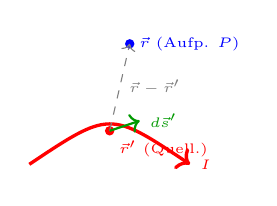
\begin{tikzpicture}[scale=0.85]
  \draw[very thick, ->, red] (-1.2,-0.3) .. controls (0,0.5) .. (1.2,-0.3) node[right]{\tiny$I$};
  \fill[red] (0,0.2) circle (2pt) node[below right]{\tiny$\vec{r}'$ (Quell.)};
  \fill[blue] (0.3,1.5) circle (2pt) node[right]{\tiny$\vec{r}$ (Aufp. $P$)};
  \draw[->,dashed,gray] (0,0.2) -- (0.3,1.5) node[midway,right]{\tiny$\vec{r}-\vec{r}'$};
  \draw[->,green!60!black,thick] (0,0.2) -- (0.45,0.35) node[right]{\tiny$d\vec{s}'$};
\end{tikzpicture}
\end{center}
\textbf{Schritte:} (1) Aufpunkt $\vec{r}$ \& Quellpunkt $\vec{r}'$ wählen\\
(2) Abstandsvektor $\vec{r}-\vec{r}'$ und Betrag berechnen\\
(3) $d\vec{s}'$ in Stromrichtung; (4) Kreuzprodukt; (5) Integrieren\\[2pt]
\textbf{Endlicher gerader Leiter} (Abstand $\rho$ von Leiter, Winkel $\alpha_1, \alpha_2$ zu den Enden):
$$H = \frac{I}{4\pi\rho}(\sin\alpha_1+\sin\alpha_2) \;\text{\textcolor{boxtitle}{[\(A/m\)]}}$$
\end{tcolorbox}

\begin{tcolorbox}[title={Unendlicher Linienleiter}]
\begin{center}
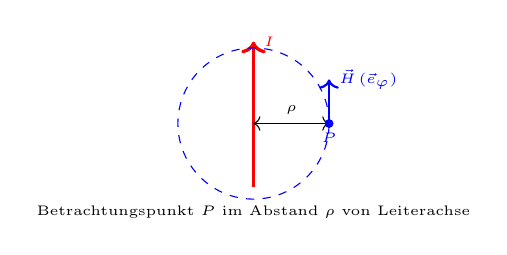
\begin{tikzpicture}[scale=0.8]
  \draw[very thick, red, ->] (0,-1) -- (0,1.3) node[right]{\tiny$I$};
  \draw[<->] (0,0) -- (1.2,0) node[midway,above]{\tiny$\rho$};
  \fill[blue] (1.2,0) circle (2pt) node[below]{\tiny$P$};
  \draw[->,blue,thick] (1.2,0) -- (1.2,0.7) node[right]{\tiny$\vec{H}$\,($\vec{e}_\varphi$)};
  \draw[dashed,blue] (0,0) circle (1.2cm);
  \node at (0,-1.4) {\tiny Betrachtungspunkt $P$ im Abstand $\rho$ von Leiterachse};
\end{tikzpicture}
\end{center}
$$\vec{H}(\rho) = \frac{I}{2\pi\rho}\vec{e}_\varphi \;\text{\textcolor{boxtitle}{[\(A/m\)]}}$$
$\rho$ \;\text{\textcolor{boxtitle}{[\(m\)]}}: Abstand des Aufpunkts $P$ von der Leiterachse\\
Ampèrescher Integrationsweg: Kreis mit Radius $\rho$ um Leiter
\end{tcolorbox}

\begin{tcolorbox}[title={Kreisschleife (z-Achse)}]
\begin{center}
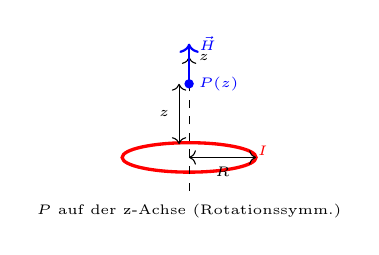
\begin{tikzpicture}[scale=0.85]
  \draw[red,very thick,->] (0,0) ellipse (1cm and 0.22cm);
  \node[red] at (1.1,0.1) {\tiny$I$};
  \draw[<->] (0,0) -- (1,0) node[midway,below]{\tiny$R$};
  \draw[dashed,->] (0,-0.5) -- (0,1.5) node[right]{\tiny$z$};
  \fill[blue] (0,1.1) circle (2pt) node[right]{\tiny$P(z)$};
  \draw[->,blue,thick] (0,1.1) -- (0,1.7) node[right]{\tiny$\vec{H}$};
  \draw[<->] (-0.15,0.2) -- (-0.15,1.1) node[midway,left]{\tiny$z$};
  \node at (0,-0.8) {\tiny$P$ auf der z-Achse (Rotationssymm.)};
\end{tikzpicture}
\end{center}
$$\vec{H}(z) = \frac{IR^2}{2(R^2+z^2)^{3/2}}\vec{e}_z \;\text{\textcolor{boxtitle}{[\(A/m\)]}}$$
Im Zentrum ($z=0$): $\vec{H} = \dfrac{I}{2R}\vec{e}_z$\\
$z$ \;\text{\textcolor{boxtitle}{[\(m\)]}}: Abstand des Aufpunkts $P$ vom Schleifenmittelpunkt auf der Achse\\
$R$ \;\text{\textcolor{boxtitle}{[\(m\)]}}: Schleifenradius
\end{tcolorbox}

\begin{tcolorbox}[title={Magnetfelder weiterer Strukturen}]
\textbf{Quadratische Schleife} (Seite $a$, Zentrum $z=0$):
$$H = \frac{2\sqrt{2}\,I}{\pi a} \;\text{\textcolor{boxtitle}{[\(A/m\)]}}$$
\textbf{Quadratische Schleife auf z-Achse:}
$$\vec{H}(z) = \frac{I}{\pi}\frac{a^2/2}{(a^2/2+z^2)\sqrt{a^2+z^2}}\vec{e}_z$$
\textbf{Spiralförmige Schleife} (Zentrum, Radien $a$ bis $3a$):
$$H = \frac{I}{2a}\ln(3)$$
\textbf{Langer Zylinder/Solenoid} ($N$ Wdg., Länge $l$):
$$H_{innen} = \frac{NI}{l} \;\text{\textcolor{boxtitle}{[\(A/m\)]}}\quad \text{(Aufpunkt im Inneren)}$$
\textbf{Toroid} (Aufpunkt im Kernbereich, Abstand $\rho$ vom Zentrum):
$$H(\rho) = \frac{NI}{2\pi\rho} \;\text{\textcolor{boxtitle}{[\(A/m\)]}}$$
\end{tcolorbox}

\begin{tcolorbox}[title={Koaxialkabel -- Magnetfeld (Ampère)}]
\begin{center}
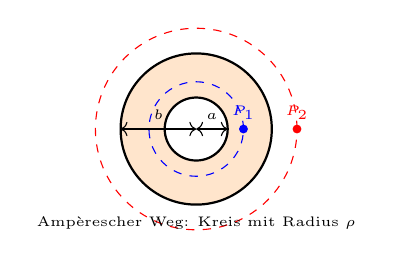
\begin{tikzpicture}[scale=0.8]
  \fill[orange!20] (0,0) circle (1.2cm);
  \fill[blue!20] (0,0) circle (0.5cm);
  \fill[white] (0,0) circle (0.5cm);
  \draw[thick] (0,0) circle (0.5cm);
  \draw[thick] (0,0) circle (1.2cm);
  \draw[<->] (0,0) -- (0.5,0) node[midway,above]{\tiny$a$};
  \draw[<->] (0,0) -- (-1.2,0) node[midway,above]{\tiny$b$};
  \fill[blue] (0.75,0) circle (2pt) node[above]{\tiny$P_1$};
  \fill[red] (1.6,0) circle (2pt) node[above]{\tiny$P_2$};
  \draw[dashed,blue] (0,0) circle (0.75cm);
  \draw[dashed,red] (0,0) circle (1.6cm);
  \node at (0,-1.5) {\tiny Ampèrescher Weg: Kreis mit Radius $\rho$};
\end{tikzpicture}
\end{center}
Aufpunkt $P$ im Abstand $\rho$ von der Achse:
$$H(\rho) = \begin{cases}
\dfrac{I}{2\pi a^2}\rho & \rho\leq a\;\text{(Innenleiter)}\\[4pt]
\dfrac{I}{2\pi\rho} & a<\rho\leq b\;\text{(Zwischenraum)}\\[4pt]
0 & \rho>b\;\text{(außen)}
\end{cases}$$
$\vec{H}$ immer in $\vec{e}_\varphi$-Richtung (Rechte-Hand-Regel)
\end{tcolorbox}

\begin{tcolorbox}[title={Stromschiene}]
\begin{center}
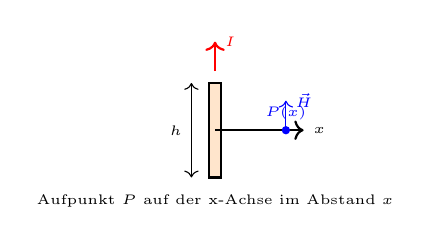
\begin{tikzpicture}[scale=0.75]
  \fill[orange!20] (-0.1,-0.8) rectangle (0.1,0.8);
  \draw[thick] (-0.1,-0.8) rectangle (0.1,0.8);
  \draw[<->] (-0.4,-0.8) -- (-0.4,0.8) node[midway,left]{\tiny$h$};
  \draw[->,red,thick] (0,1) -- (0,1.5) node[right]{\tiny$I$};
  \draw[->,thick] (0,0) -- (1.5,0) node[right]{\tiny$x$};
  \fill[blue] (1.2,0) circle (2pt) node[above]{\tiny$P(x)$};
  \draw[->,blue] (1.2,0) -- (1.2,0.5) node[right]{\tiny$\vec{H}$};
  \node at (0,-1.2) {\tiny Aufpunkt $P$ auf der x-Achse im Abstand $x$};
\end{tikzpicture}
\end{center}
$$\vec{H}(x) = \frac{I}{\pi h}\arctan\!\left(\frac{h}{2x}\right)\vec{e}_y \;\text{\textcolor{boxtitle}{[\(A/m\)]}}$$
Grenzwert $x\ll h$ (nah, wirkt wie $\infty$-Fläche): $\vec{H}=\dfrac{I}{2h}\vec{e}_y$\\
Grenzwert $h\to0$ (wirkt wie Linienleiter): $\vec{H}=\dfrac{I}{2\pi x}\vec{e}_y$
\end{tcolorbox}

\begin{tcolorbox}[title={Grenzbedingungen Magnetostatik}]
\begin{center}
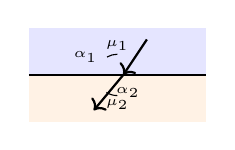
\begin{tikzpicture}[scale=0.75]
  \fill[blue!10] (-1.5,0) rectangle (1.5,0.8);
  \fill[orange!10] (-1.5,-0.8) rectangle (1.5,0);
  \draw[thick] (-1.5,0) -- (1.5,0);
  \node at (0,0.5) {\tiny$\mu_1$};\node at (0,-0.5) {\tiny$\mu_2$};
  \draw[->,thick] (0.5,0.6) -- (0.1,0);
  \draw[->,thick] (0.1,0) -- (-0.4,-0.6);
  \draw (0,0.35) arc(90:120:0.35) node[left]{\tiny$\alpha_1$};
  \draw (0,-0.35) arc(270:238:0.35) node[right]{\tiny$\alpha_2$};
\end{tikzpicture}
\end{center}
\textbf{Normal} (B-Feld stetig): $B_{1n} = B_{2n}$\\
\textbf{Tangential} (H-Feld springt bei Flächenstrom):
$$\vec{n}\times(\vec{H}_2-\vec{H}_1) = \vec{J}_F \;\text{\textcolor{boxtitle}{[\(A/m\)]}}$$
Ohne Flächenstrom: $H_{1t} = H_{2t}$\\[2pt]
\textbf{Brechungsgesetz:} $\dfrac{\tan\alpha_1}{\tan\alpha_2} = \dfrac{\mu_1}{\mu_2}$
\end{tcolorbox}

\begin{tcolorbox}[title={Induktivitäten -- alle Geometrien}]
$L = N\Phi/I = \Psi/I$ \;\text{\textcolor{boxtitle}{[\(H = Vs/A\)]}};\quad $W_m = \tfrac{1}{2}LI^2$ \;\text{\textcolor{boxtitle}{[\(J\)]}}\\[3pt]
\textbf{Zylinderspule:} $L = \mu_0\mu_r N^2 A/l$\\
\textbf{Toroid (Rechteckquerschnitt, Höhe $h$):}
$$L = \frac{\mu_0\mu_r N^2 h}{2\pi}\ln\!\left(\frac{r_a}{r_i}\right)$$
\textbf{Koaxialkabel:} $L = \dfrac{\mu_0\mu_r l}{2\pi}\ln\!\left(\dfrac{r_a}{r_i}\right)$\\
\textbf{Doppelleitung} (Drahtradius $r$, Abstand $d$): $L' = \dfrac{\mu_0}{\pi}\ln(d/r)$ \;\text{\textcolor{boxtitle}{[\(H/m\)]}}\\[2pt]
\textbf{Kreisschleife} ($R\gg r$, Drahtradius $r$):
$$L \approx \mu_0 R\!\left(\ln\frac{8R}{r}-2\right)$$
\end{tcolorbox}

\begin{tcolorbox}[title={Gegeninduktivität \& magnetische Kopplung}]
$$M = \frac{\Phi_{21}}{I_1} = \frac{\mu_0}{4\pi}\oint_{C_1}\oint_{C_2}\frac{d\vec{s}_1\cdot d\vec{s}_2}{|\vec{r}_1-\vec{r}_2|} \;\text{\textcolor{boxtitle}{[\(H\)]}}$$
$M_{12}=M_{21}=M$ (Reziprozität)\\
Kopplungskoeffizient: $k = M/\sqrt{L_1 L_2}$;\quad $0\leq k\leq1$\\
Gesamtenergie: $W_m = \tfrac{1}{2}L_1 I_1^2 + MI_1I_2 + \tfrac{1}{2}L_2 I_2^2$\\
Fluss durch Schleife 2: $\Phi_{21} = \iint_{A_2}\vec{B}_1\cdot d\vec{A}_2$
\end{tcolorbox}

%=============================================================
\section*{5. Induktion \& Quasistationäre Felder}
%=============================================================

\begin{tcolorbox}[title={Faradaysches Induktionsgesetz}]
$$U_{ind} = \oint\vec{E}\cdot d\vec{s} = -\frac{d\Phi}{dt} \;\text{\textcolor{boxtitle}{[\(V\)]}}$$
$\Phi = \iint\vec{B}\cdot d\vec{A}$ \;\text{\textcolor{boxtitle}{[\(Wb = Vs\)]}}: magnetischer Fluss\\[4pt]
\begin{center}
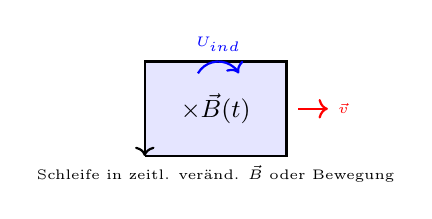
\begin{tikzpicture}[scale=0.75]
  \fill[blue!10] (-1.2,-0.8) rectangle (1.2,0.8);
  \draw[thick,->] (-1.2,-0.8) -- (1.2,-0.8) -- (1.2,0.8) -- (-1.2,0.8) -- (-1.2,-0.8);
  \node at (0,0) {\small$\times\vec{B}(t)$};
  \draw[->,thick,blue] (-0.3,0.6) arc(150:30:0.4) node[midway,above]{\tiny$U_{ind}$};
  \draw[->,thick,red] (1.4,0) -- (1.9,0) node[right]{\tiny$\vec{v}$};
  \node at (0,-1.1) {\tiny Schleife in zeitl. veränd. $\vec{B}$ oder Bewegung};
\end{tikzpicture}
\end{center}
\textbf{Transformatorisch} (ruhende Schleife):
$$U_{ind} = -\iint_A\frac{\partial\vec{B}}{\partial t}\cdot d\vec{A}$$
\textbf{Bewegungsinduktion} (konst. $\vec{B}$, bewegter Leiter):
$$U_{ind} = \int_C(\vec{v}\times\vec{B})\cdot d\vec{s}$$
\textbf{Allgemein:} $U_{ind} = -\iint_A\dfrac{\partial\vec{B}}{\partial t}\cdot d\vec{A} + \oint(\vec{v}\times\vec{B})\cdot d\vec{s}$\\[3pt]
\textbf{Vorgehen:}\\
1. Fläche $A$, $d\vec{A}$ und Umlaufsinn (RHR) definieren\\
2. $\Phi(t) = \iint\vec{B}\cdot d\vec{A}$ berechnen\\
3. $U_{ind} = -d\Phi/dt$; Vorzeichen prüfen!
\end{tcolorbox}

\begin{tcolorbox}[title={Induktionsspannungen typischer Aufgaben}]
\textbf{Ruhende Schleife nahe $\infty$-Linienleiter} $i(t)$:
$$U_{ind} = -\frac{\mu_0 h}{2\pi}\frac{di}{dt}\ln\!\left(\frac{y_0+b}{y_0}\right)$$
$h$: Schleifenhöhe;\quad $b$: Breite;\quad $y_0$: nächster Abstand\\[2pt]
\textbf{Bewegte Schleife} ($v_0$), Gleichstrom $I_0$:
$$U_{ind} = \frac{\mu_0 I_0 v_0 h}{2\pi}\cdot\frac{b}{(y_0+v_0t)(y_0+v_0t+b)}$$
\textbf{Rotierende Schleife} (Fläche $A$, $B_0$):
$$\Phi(t) = B_0 A\cos(\omega t),\quad U_{ind} = B_0 A\omega\sin(\omega t)$$
\textbf{Rechteckschleife $2a\times2b$} (rotiert, Feld $H_0$):
$$U_{ind} = 4ab\mu_0 H_0\omega\sin(\omega t)$$
\textbf{Zwei senkrechte $\infty$-Linienleiter} (x- und y-Achse, je $i(t)$):
$$\vec{B}_{ges} = \frac{\mu_0 i(t)}{2\pi}\!\left(\frac{\vec{e}_z}{y} - \frac{\vec{e}_z}{x}\right)$$
Daraus $\Phi$ durch Rechteckrahmen integrieren, dann ableiten.
\end{tcolorbox}

\begin{tcolorbox}[title={EQS vs. MQS -- Vergleich}]
\begin{tabular}{@{}lll@{}}
\toprule
Aspekt & \textbf{EQS} & \textbf{MQS}\\
\midrule
Vernachlässigt & $\partial_t\vec{B}\approx0$ & $\partial_t\vec{D}\approx0$\\
Hauptfeld & $\vec{E}$, $\vec{D}$ & $\vec{H}$, $\vec{B}$\\
Gleichung & Laplace/Poisson & Diffusionsgl.\\
Physik & E sofort verteilt & B dringt langsam ein\\
Beispiel & Kondensator & Trafo, Skin\\
\bottomrule
\end{tabular}
\end{tcolorbox}

\begin{tcolorbox}[title={Skin-Effekt \& Eindringtiefe}]
\begin{center}
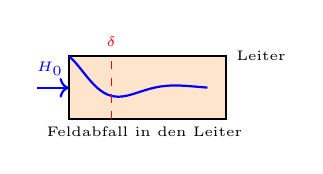
\begin{tikzpicture}[scale=0.8]
  \fill[orange!20] (0,-0.5) rectangle (2.5,0.5);
  \draw[thick] (0,-0.5) rectangle (2.5,0.5) node[right]{\tiny Leiter};
  \draw[thick,blue,->] (-0.5,0) -- (0,0);
  \draw[blue,thick,domain=0:2.2,samples=40]
    plot(\x, {0.5*exp(-1.5*\x)*cos(200*\x)});
  \draw[dashed,red] (0.67,-0.5) -- (0.67,0.5) node[above]{\tiny$\delta$};
  \node[blue] at (-0.3,0.3) {\tiny$H_0$};
  \node at (1.2,-0.7) {\tiny Feldabfall in den Leiter};
\end{tikzpicture}
\end{center}
Eindringtiefe \;\text{\textcolor{boxtitle}{[\(m\)]}}: $\delta = \sqrt{\dfrac{2}{\omega\mu\kappa}}$\\
$\omega$ \;\text{\textcolor{boxtitle}{[\(rad/s\)]}}: Kreisfreq.;\quad $\mu$ \;\text{\textcolor{boxtitle}{[\(H/m\)]}}: Permeab.;\quad $\kappa$ \;\text{\textcolor{boxtitle}{[\(S/m\)]}}: Leitf.\\[3pt]
Feldverlauf: $\vec{H}(x,t)=H_0 e^{-x/\delta}\cos(\omega t-x/\delta)\vec{e}_y$\\
$R_{AC}\approx R_{DC}\cdot d/(4\delta)$ \quad für $d\gg\delta$\\
Kupfer: $\delta\approx 66/\sqrt{f\,[\text{Hz}]}$ mm
\end{tcolorbox}

\begin{tcolorbox}[title={Diffusionsgleichung (MQS)}]
$\partial_t\vec{D}\approx0$ eingesetzt in Maxwell $\Rightarrow$:
$$\Delta\vec{H} = \kappa\mu\frac{\partial\vec{H}}{\partial t} \;\text{\textcolor{boxtitle}{[\(A/m^3\)]}}$$
\textbf{Harmonisch} ($e^{j\omega t}$): $\Delta\vec{H} = j\omega\kappa\mu\,\vec{H}$\\
Komplexe Wellenzahl: $\underline{k}^2 = j\omega\mu\kappa$;\\
Lösung (1D, Halbraum): $H(x) = H_0\,e^{-(1+j)x/\delta}$
\end{tcolorbox}

\begin{tcolorbox}[title={Komplexe Zeiger / Phasoren}]
Zeitharmonisch: $f(t) = \hat{F}\cos(\omega t+\varphi_0) = \text{Re}\{\underline{F}\,e^{j\omega t}\}$\\
Phasor: $\underline{F} = \hat{F}e^{j\varphi_0}$ \quad (komplex, zeitunabhängig)\\
Zeitableitung: $\partial/\partial t \longrightarrow j\omega$\\[3pt]
Maxwell in Phasorform:
$$\text{rot}\,\underline{\vec{E}} = -j\omega\underline{\vec{B}},\quad \text{rot}\,\underline{\vec{H}} = \underline{\vec{J}} + j\omega\underline{\vec{D}}$$
Komplexe Permittivität: $\underline{\varepsilon} = \varepsilon\!\left(1 - j\dfrac{\kappa}{\omega\varepsilon}\right)$
\end{tcolorbox}

%=============================================================
\section*{6. Energien, Kräfte \& Poynting}
%=============================================================

\begin{tcolorbox}[title={Elektromagnetische Energiedichten}]
Elektrisch: $w_e = \tfrac{1}{2}\vec{E}\cdot\vec{D} = \tfrac{1}{2}\varepsilon E^2$ \;\text{\textcolor{boxtitle}{[\(J/m^3\)]}}\\
Magnetisch: $w_m = \tfrac{1}{2}\vec{H}\cdot\vec{B} = \tfrac{1}{2}\mu H^2 = B^2/(2\mu)$ \;\text{\textcolor{boxtitle}{[\(J/m^3\)]}}\\[3pt]
Gesamtenergie: $W_e = \tfrac{1}{2}CU^2 = Q^2/(2C)$ \;\text{\textcolor{boxtitle}{[\(J\)]}}\\
Gesamtenergie: $W_m = \tfrac{1}{2}LI^2$ \;\text{\textcolor{boxtitle}{[\(J\)]}}\\[3pt]
\textbf{Poynting-Vektor:} $\vec{S} = \vec{E}\times\vec{H}$ \;\text{\textcolor{boxtitle}{[\(W/m^2\)]}}\\
Leistungsfluss: $P = \iint_A\vec{S}\cdot d\vec{A}$ \;\text{\textcolor{boxtitle}{[\(W\)]}}\\[3pt]
\textbf{Energieerhaltung (Poynting-Theorem):}
$$-\frac{\partial}{\partial t}(w_e+w_m) = \nabla\cdot\vec{S} + \underbrace{\vec{J}\cdot\vec{E}}_{\text{Verluste}}$$
\textbf{Zeitgemittelt} (harmonisch): $\langle\vec{S}\rangle = \tfrac{1}{2}\,\text{Re}\{\underline{\vec{E}}\times\underline{\vec{H}}^*\}$
\end{tcolorbox}

%=============================================================
\section*{7. Elektromagnetische Wellen}
%=============================================================

\begin{tcolorbox}[title={Wellengleichung \& ebene Welle}]
\textbf{Wellengleichung} (Vakuum, $\rho_V=0$, $\vec{J}=0$):
$$\Delta\vec{E} - \mu_0\varepsilon_0\frac{\partial^2\vec{E}}{\partial t^2} = 0,\quad c = \frac{1}{\sqrt{\mu_0\varepsilon_0}}$$
\begin{center}
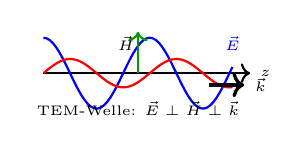
\begin{tikzpicture}[scale=0.75]
  \draw[->,thick] (0,0) -- (3.5,0) node[right]{\tiny$z$};
  \draw[blue,thick,domain=0:3.2,samples=60] plot(\x,{0.6*cos(200*\x)});
  \draw[red,thick,domain=0:3.2,samples=60] plot(\x,{0.6*sin(200*\x)*0.4}) node[right]{};
  \node[blue] at (3.2,0.5) {\tiny$\vec{E}$};
  \draw[->,thick,green!60!black] (1.6,0) -- (1.6,0.7);
  \node at (1.4,0.5) {\tiny$\vec{H}$};
  \draw[->,very thick] (2.8,-0.2) -- (3.4,-0.2) node[right]{\tiny$\vec{k}$};
  \node at (1.6,-0.6) {\tiny TEM-Welle: $\vec{E}\perp\vec{H}\perp\vec{k}$};
\end{tikzpicture}
\end{center}
Lösung: $\vec{E}(z,t) = E_0\cos(\omega t - kz)\vec{e}_x$\\
Wellenzahl: $k = \omega/c = 2\pi/\lambda$ \;\text{\textcolor{boxtitle}{[\(1/m\)]}}\\
Wellenlänge: $\lambda = c/f$ \;\text{\textcolor{boxtitle}{[\(m\)]}};\quad Periode: $T = 1/f$ \;\text{\textcolor{boxtitle}{[\(s\)]}}\\[3pt]
\textbf{Wellenimpedanz:}
$$Z_0 = \sqrt{\frac{\mu_0}{\varepsilon_0}} = 377\,\Omega;\quad Z = Z_0\sqrt{\frac{\mu_r}{\varepsilon_r}}$$
$E = Z\cdot H$;\quad $\vec{H} = \frac{1}{Z}\vec{e}_k\times\vec{E}$\\[3pt]
\textbf{Verlustbehaftetes Medium} ($\kappa\neq0$):
$$\vec{E} = E_0 e^{-\alpha z}\cos(\omega t-\beta z)\vec{e}_x$$
$\alpha$ \;\text{\textcolor{boxtitle}{[\(Np/m\)]}}: Dämpfung;\quad $\beta$ \;\text{\textcolor{boxtitle}{[\(rad/m\)]}}: Phasenkonstante\\
Guter Leiter ($\kappa\gg\omega\varepsilon$): $\alpha\approx\beta\approx 1/\delta$
\end{tcolorbox}

\begin{tcolorbox}[title={Reflexion \& Brechung an Grenzflächen}]
\begin{center}
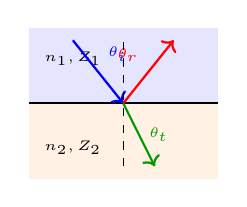
\begin{tikzpicture}[scale=0.8]
  \fill[blue!10] (-1.5,0) rectangle (1.5,1.2);
  \fill[orange!10] (-1.5,-1.2) rectangle (1.5,0);
  \draw[thick] (-1.5,0) -- (1.5,0);
  \node at (-0.8,0.7) {\tiny$n_1, Z_1$};
  \node at (-0.8,-0.7) {\tiny$n_2, Z_2$};
  \draw[->,thick,blue] (-0.8,1) -- (0,0) node[midway,above right]{\tiny$\theta_i$};
  \draw[->,thick,red] (0,0) -- (0.8,1) node[midway,above left]{\tiny$\theta_r$};
  \draw[->,thick,green!60!black] (0,0) -- (0.5,-1) node[midway,right]{\tiny$\theta_t$};
  \draw[dashed] (0,-1) -- (0,1);
\end{tikzpicture}
\end{center}
\textbf{Snellius:} $n_1\sin\theta_i = n_2\sin\theta_t$;\quad $n=c/v_{ph}=\sqrt{\varepsilon_r\mu_r}$\\[3pt]
\textbf{Reflexion senkrechter Einfall} ($\theta_i=0$):
$$r = \frac{Z_2-Z_1}{Z_2+Z_1},\quad t = \frac{2Z_2}{Z_2+Z_1}$$
\textbf{Stehende Welle} (ideal. Leiter, $Z_2=0$):
$$E(z,t) = 2E_0\sin(kz)\sin(\omega t)$$
\end{tcolorbox}

%=============================================================
\section*{8. Wichtige Konstanten \& Hilfsmittel}
%=============================================================

\begin{tcolorbox}[title={Konstanten \& Materialdaten}]
$\varepsilon_0 = 8{,}854\cdot10^{-12}$ \;\text{\textcolor{boxtitle}{[\(F/m\)]}};\quad $\mu_0 = 4\pi\cdot10^{-7}$ \;\text{\textcolor{boxtitle}{[\(H/m\)]}}\\
$c = 2{,}998\cdot10^8$ \;\text{\textcolor{boxtitle}{[\(m/s\)]}};\quad $Z_0 = 376{,}7$ \;\text{\textcolor{boxtitle}{[\(\Omega\)]}}\\
$e = 1{,}602\cdot10^{-19}$ \;\text{\textcolor{boxtitle}{[\(C\)]}}\\[3pt]
\textbf{Leitfähigkeiten $\kappa$:}\\
Kupfer: $5{,}8\cdot10^7$ S/m;\quad Alu: $3{,}8\cdot10^7$ S/m\\
Eisen: $\approx10^7$ S/m;\quad Silizium: $\approx10^{-4}$ S/m\\[3pt]
\textbf{Relative Permittivitäten $\varepsilon_r$:}\\
Vakuum/Luft: 1;\quad Glas: 4--8;\quad Wasser: 80
\end{tcolorbox}

\begin{tcolorbox}[title={Nützliche Integrale}]
$\displaystyle\int\frac{dz}{(a^2+z^2)^{3/2}} = \frac{z}{a^2\sqrt{a^2+z^2}} + C$\\[3pt]
$\displaystyle\int\frac{z\,dz}{(a^2+z^2)^{3/2}} = -\frac{1}{\sqrt{a^2+z^2}} + C$\\[3pt]
$\displaystyle\int\frac{dz}{a^2+z^2} = \frac{1}{a}\arctan\!\left(\frac{z}{a}\right)+C$\\[3pt]
$\displaystyle\int\frac{z\,dz}{a^2+z^2} = \frac{1}{2}\ln(a^2+z^2)+C$\\[3pt]
$\displaystyle\int\frac{dz}{\sqrt{a^2+z^2}} = \ln(z+\sqrt{a^2+z^2})+C$\\[3pt]
$\displaystyle\int\frac{dz}{az+b} = \frac{1}{a}\ln|az+b|+C$\\[3pt]
$\int_0^\pi\sin\theta\,d\theta = 2$;\quad $\int_0^\pi\sin^2\theta\,d\theta = \pi/2$\\[2pt]
$\int_0^{2\pi}d\varphi = 2\pi$;\quad $\int_0^{2\pi}\cos^2\varphi\,d\varphi = \pi$
\end{tcolorbox}

\begin{tcolorbox}[title={Kreuzprodukt \& Vektorregeln}]
\textbf{Kartesisch:} $\vec{e}_x\times\vec{e}_y=\vec{e}_z$;\; $\vec{e}_y\times\vec{e}_z=\vec{e}_x$;\; $\vec{e}_z\times\vec{e}_x=\vec{e}_y$\\
\textbf{Zylinder:} $\vec{e}_\rho\times\vec{e}_\varphi=\vec{e}_z$;\; $\vec{e}_\varphi\times\vec{e}_z=\vec{e}_\rho$;\; $\vec{e}_z\times\vec{e}_\rho=\vec{e}_\varphi$\\[3pt]
$|\vec{a}\times\vec{b}| = |\vec{a}||\vec{b}|\sin\angle(\vec{a},\vec{b})$;\quad $\vec{a}\times\vec{b} = -\vec{b}\times\vec{a}$\\
\textbf{BAC-CAB:} $\vec{a}\times(\vec{b}\times\vec{c}) = \vec{b}(\vec{a}\cdot\vec{c})-\vec{c}(\vec{a}\cdot\vec{b})$
\end{tcolorbox}

\begin{tcolorbox}[title={Analogietabelle der Feldtypen}]
\begin{tabular}{@{}p{2cm}p{2cm}p{2cm}@{}}
\toprule
\textbf{Elektrostatik} & \textbf{Magnetostatik} & \textbf{Strömungsfeld}\\
\midrule
$\vec{E}$ \;\text{\textcolor{boxtitle}{[\(V/m\)]}} & $\vec{H}$ \;\text{\textcolor{boxtitle}{[\(A/m\)]}} & $\vec{E}$ \;\text{\textcolor{boxtitle}{[\(V/m\)]}}\\
$\vec{D}=\varepsilon\vec{E}$ & $\vec{B}=\mu\vec{H}$ & $\vec{J}=\kappa\vec{E}$\\
$\rho_V$ \;\text{\textcolor{boxtitle}{[\(C/m^3\)]}} & $\vec{J}$ \;\text{\textcolor{boxtitle}{[\(A/m^2\)]}} & --\\
$C=Q/U$ & $L=\Psi/I$ & $G=1/R$\\
$W_e=\tfrac{1}{2}CU^2$ & $W_m=\tfrac{1}{2}LI^2$ & $P=UI$\\
$\phi$ & $\vec{A}$ & $\phi$\\
Laplace & Poisson & Laplace\\
\bottomrule
\end{tabular}
\end{tcolorbox}

\begin{tcolorbox}[title={Materialeigenschaften -- Definitionen}]
\textbf{Homogen:} $\varepsilon, \mu, \kappa$ unabhängig vom \textit{Ort}\\
\textbf{Isotrop:} $\varepsilon, \mu, \kappa$ unabhängig von der \textit{Richtung} (Skalar, kein Tensor)\\
\textbf{Linear:} $\vec{D}\propto\vec{E}$ (keine Sättigung, kein Hystereseeffekt)\\
\textbf{Ferromagenetikum:} $\mu_r\gg1$, Hysterese, Remanenz\\
\textbf{Paramagnetikum:} $\mu_r$ leicht $>1$\\
\textbf{Diamagnetikum:} $\mu_r$ leicht $<1$
\end{tcolorbox}

\begin{tcolorbox}[title={Lösungsstrategien -- Schnellübersicht}]
\begin{tabular}{@{}ll@{}}
\toprule
Symmetrie & Methode\\
\midrule
Kugelsymm. & Gauß ($\vec{e}_r$, Kugelschale)\\
Zylindersymm. & Gauß / Ampère ($\vec{e}_\rho$, Zylindermantel)\\
Plattensymm. & Gauß ($\vec{e}_z$, Quaderbox)\\
Keine Symm. & Superposition oder Laplace lösen\\
Randwertprob. & Laplace + RB einsetzen\\
Leiter in Nähe & Spiegelungsmethode\\
Wechselfeld & Faraday + Phasoren\\
\bottomrule
\end{tabular}\\[3pt]
\textbf{$R$ aus Feldern:}
$R = \dfrac{\int\vec{E}\cdot d\vec{s}}{\int\kappa\vec{E}\cdot d\vec{A}}$\\[3pt]
\textbf{$C$ aus Feldern:}
$C = \dfrac{\varepsilon\oint\vec{E}\cdot d\vec{A}}{\int\vec{E}\cdot d\vec{s}}$
\end{tcolorbox}

%=============================================================
\section*{Ergänzungen aus weiteren Unterlagen}
%=============================================================

\begin{tcolorbox}[title={Reflexion, Transmission und Brewster-Winkel}]
\textbf{k-Reflexionsfaktor:}\\
$r_k = \frac{\vec{n}\circ(\vec{k}_{in}-\vec{k}_{tr})}{\vec{n}\circ(\vec{k}_{in}+\vec{k}_{tr})}$\\
\textbf{Dielektrisch / Magnetisch:}\\
$r_\epsilon = \frac{\epsilon_{in}-\epsilon_{tr}}{\epsilon_{in}+\epsilon_{tr}}$,\quad $r_\mu = \frac{\mu_{in}-\mu_{tr}}{\mu_{in}+\mu_{tr}}$\\[3pt]
\textbf{Brewster-Winkel Bedingungen:}\\
TE-Welle: $r_k = r_\mu$\\
TM-Welle: $r_k = r_\epsilon$\\[3pt]
\textbf{Intensitätsfaktoren (Poynting):}\\
$R = -\frac{\vec{n}\circ\vec{S}_{ref}}{\vec{n}\circ\vec{S}_{in}}$,\quad $T = \frac{\vec{n}\circ\vec{S}_{tr}}{\vec{n}\circ\vec{S}_{in}}$
\end{tcolorbox}

\begin{tcolorbox}[title={Wechselstrom \& Drehstrom (Leistung)}]
\textbf{Leistungsarten:}\\
Scheinleistung: $S = U \cdot I$ \unitbox{VA}\\
Wirkleistung: $P = U \cdot I \cdot \cos\varphi$ \unitbox{W}\\
Blindleistung: $Q = U \cdot I \cdot \sin\varphi$ \unitbox{var}\\[3pt]
\textbf{Drehstrom (Transformator):}\\
$P = \sqrt{3} \cdot U_p \cdot I_p \cdot \cos\varphi_p = \sqrt{3} \cdot U_s \cdot I_s \cdot \cos\varphi_s + P_v$\\
$Q = \sqrt{3} \cdot U_p \cdot I_p \cdot \sin\varphi_p = \sqrt{3} \cdot U_s \cdot I_s \cdot \sin\varphi_s + P_v$\\
$S = \sqrt{3} \cdot U_p \cdot I_p = \sqrt{3} \cdot U_s \cdot I_s + P_v$
\end{tcolorbox}

\begin{tcolorbox}[title={Kugelfunktionen (Additionstheorem)}]
\textbf{Kugelflächenfunktionen:}\\
$g(\vartheta, \varphi) = Y_{lm}(\vartheta, \varphi)$\\
Entwicklung für Legendre-Polynome:\\
$P_l(\cos \alpha) = \sum_{m=-l}^{l} b_{lm} Y_{lm}(\vartheta, \varphi)$\\[3pt]
\textbf{Integration über Raumwinkel:}\\
$\int Y_{lm}(\vartheta, \varphi) Y_{l0}^*(\alpha, \beta) d\Omega = a_{l0}$
\end{tcolorbox}

\begin{tcolorbox}[title={Ergänzende Modelle (aus Bildreferenzen)}]
\textbf{Leitungstheorie (Telegraphengleichung):}\\
$\frac{\partial U}{\partial x} = -R' I - L' \frac{\partial I}{\partial t}$\\
$\frac{\partial I}{\partial x} = -G' U - C' \frac{\partial U}{\partial t}$\\[3pt]
\textbf{Hertzscher Dipol (Fernfeld):}\\
$\underline{E}_\vartheta = j \omega \mu \frac{\underline{I} l}{4 \pi r} \sin\vartheta e^{-jkr}$\\
$\underline{H}_\varphi = \frac{\underline{E}_\vartheta}{Z_0}$\\[3pt]
\textbf{Wellenleiter (Rechteckhohlleiter):}\\
Grenzfrequenz: $f_c = \frac{c}{2} \sqrt{(\frac{m}{a})^2 + (\frac{n}{b})^2}$
\end{tcolorbox}

%=============================================================
\section*{9. Ergänzende Skizzen \& Beziehungen (aus Vorlesungsskript)}
%=============================================================

\begin{tcolorbox}[title={Vergleich: Elektrostatik und Strömungsfeld}]
\begin{tabular}{@{}p{3.5cm}p{3.5cm}@{}}
\toprule
\textbf{Elektrostatik} & \textbf{Strömungsfeld} \\
\midrule
$\vec{D} = \epsilon \cdot \vec{E}$ & $\vec{J} = \kappa \cdot \vec{E}$ \\
$\text{div}\,\vec{D} = \rho_V$ & $\text{div}\,\vec{J} = 0$ \\
$D_{2n} - D_{1n} = 0$ & $J_{2n} - J_{1n} = 0$ \\
$\frac{D_{2t}}{\epsilon_2} = \frac{D_{1t}}{\epsilon_1}$ & $\frac{J_{2t}}{\kappa_2} = \frac{J_{1t}}{\kappa_1}$ \\
$C = \frac{Q}{U}$ & $G = \frac{I}{U}$ \\
$\vec{E} = -\text{grad}\,\phi$ & $\vec{E} = -\text{grad}\,\phi$ \\
$\Delta\phi = -\frac{\rho_V}{\epsilon}$ & $\Delta\phi = 0$ \\
$E_{2t} - E_{1t} = 0$ & $E_{2t} - E_{1t} = 0$ \\
\bottomrule
\end{tabular}
\end{tcolorbox}

\begin{tcolorbox}[title={Skizzen: Induktion, Gegeninduktivität \& Skin-Effekt}]
\textbf{Skin-Effekt (Wirbelströme):}\\
\begin{center}
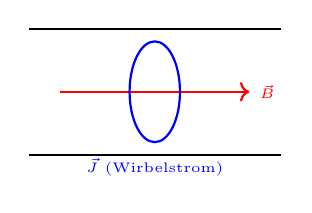
\begin{tikzpicture}[scale=0.8]
  \draw[thick] (-2, 1) -- (2, 1);
  \draw[thick] (-2, -1) -- (2, -1);
  \draw[->, red, thick] (-1.5, 0) -- (1.5, 0) node[right]{\tiny $\vec{B}$};
  \draw[->, blue, thick] (0, 0) ellipse (0.4 and 0.8);
  \node[blue] at (0, -1.2) {\tiny $\vec{J}$ (Wirbelstrom)};
\end{tikzpicture}
\end{center}
\vspace{3mm}

\textbf{Gegeninduktivität (Zwei Leiterschleifen):}\\
\begin{center}
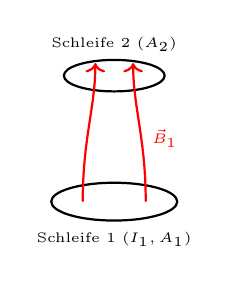
\begin{tikzpicture}[scale=0.8]
  \draw[thick] (0,0) ellipse (1 and 0.3);
  \draw[thick] (0,2) ellipse (0.8 and 0.25);
  \node at (0, -0.6) {\tiny Schleife 1 ($I_1, A_1$)};
  \node at (0, 2.5) {\tiny Schleife 2 ($A_2$)};
  \draw[->, red, thick] (-0.5, 0) .. controls (-0.5, 1) and (-0.3, 1.5) .. (-0.3, 2.2);
  \draw[->, red, thick] (0.5, 0) .. controls (0.5, 1) and (0.3, 1.5) .. (0.3, 2.2);
  \node[red] at (0.8, 1) {\tiny $\vec{B}_1$};
\end{tikzpicture}
\end{center}
\vspace{3mm}

\textbf{Induktion durch Relativbewegung:}\\
\begin{center}
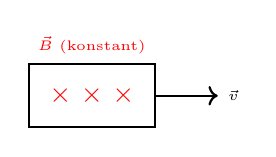
\begin{tikzpicture}[scale=0.8]
  \draw[thick] (0,0) rectangle (2,1);
  \draw[->, thick] (2, 0.5) -- (3, 0.5) node[right]{\tiny $\vec{v}$};
  \foreach \x in {0.5, 1.0, 1.5} {
    \node[red] at (\x, 0.5) {$\times$};
  }
  \node[red] at (1, 1.3) {\tiny $\vec{B}$ (konstant)};
\end{tikzpicture}
\end{center}
\end{tcolorbox}

\end{multicols*}
\end{document}